% !TeX root = ../Project2.tex
\section{Results}
\label{sec:results}
\subsection{NeuralNetRegressor}
\subsubsection{First CV GridSearch}
\begin{figure}[htbp]
    \centering
    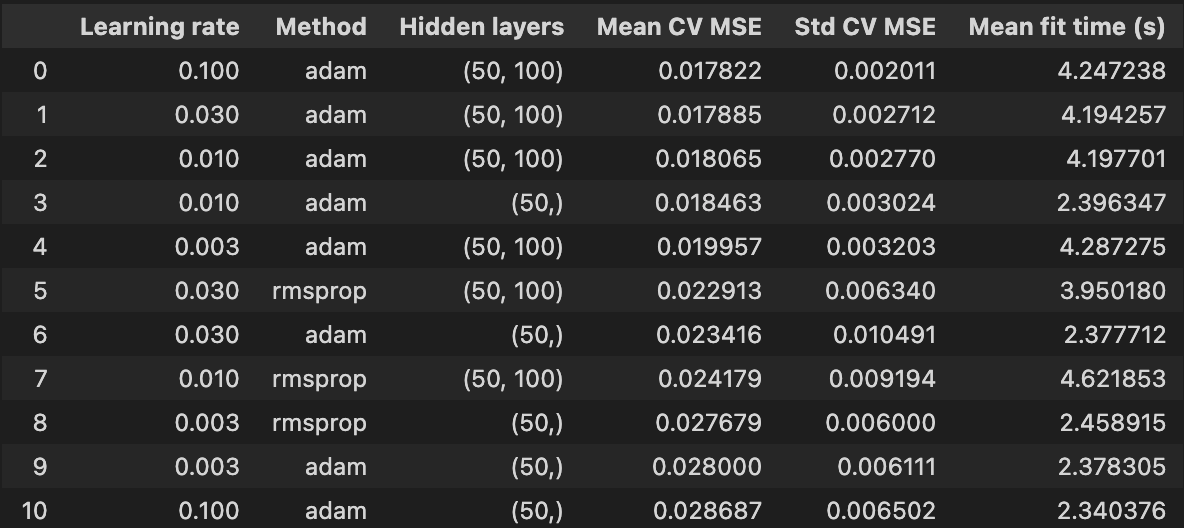
\includegraphics[width=\linewidth]{Results/Regressor/MS11.png}
    \caption{$\mathbf{First CVGridSearch}:$ First 10 model scores with standard error and mean fit time.}
    \label{fig:MS11}
\end{figure}
The first GridSearchCV results are plotted in a heatmap.
As seen from the heatmap, the best model within one se has one hidden layer with 50 nodes, adam as gradient descent method and a
learning rate of $0.01$. The model with the lowest score has a higher learning rate of $0.1$ and two hidden layers with 50 and 100 nodes.
\begin{figure}[htbp]
    \centering
    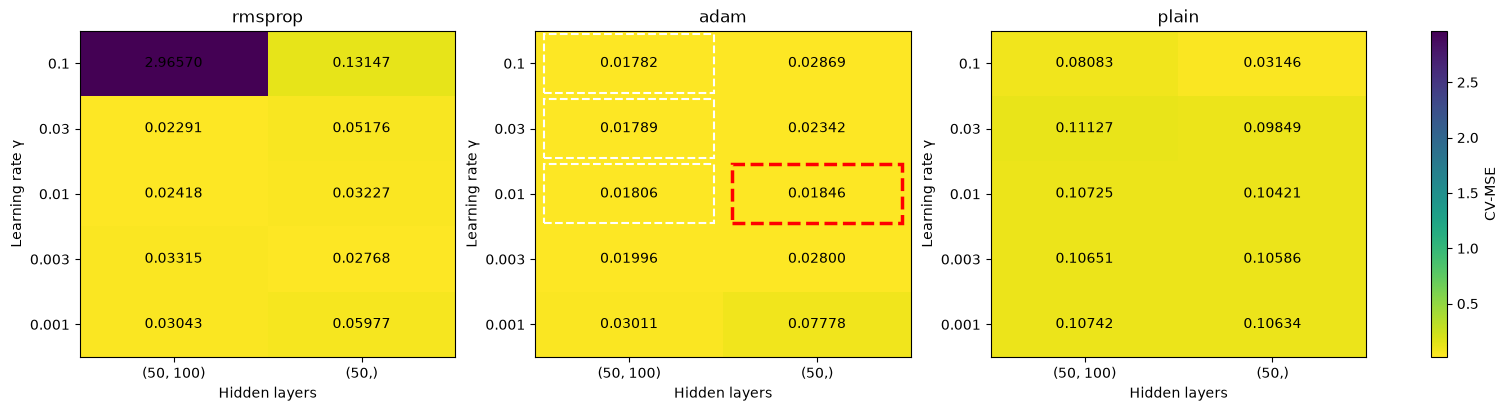
\includegraphics[width=\linewidth]{Results/Regressor/HM1.png}
    \caption{$\mathbf{Heatmap}$ for methods rmsprop, adam and plain, showing learning rate and hidden layers as axis values,
    with the color bar showing cross validation MSE. The dotted lines show all models within one standard error of the best,
    and the red dotted line shows the chosen model, which is the model with least hidden layers and nodes}
    \label{fig:HM1}
\end{figure}
\subsubsection{OLS comparison and test set}
\begin{figure}[htbp]
    \centering
    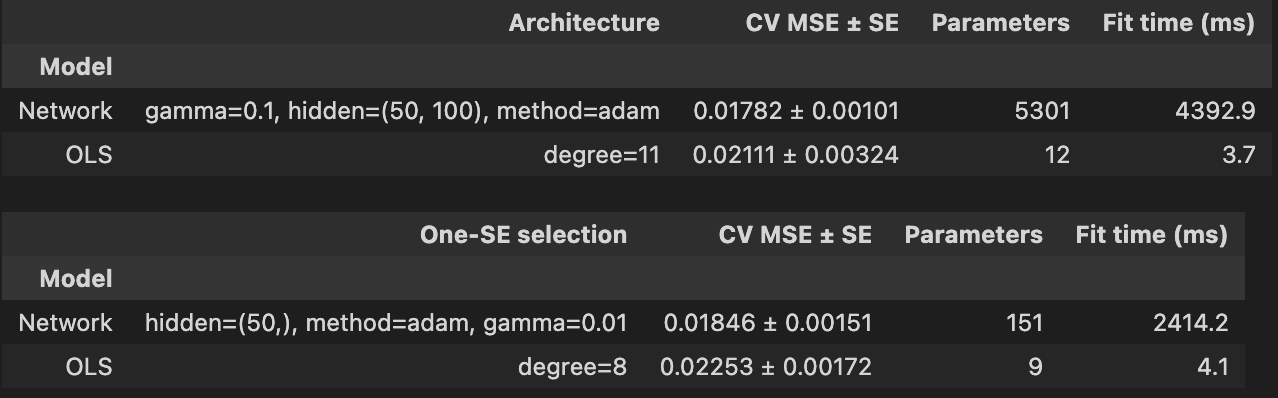
\includegraphics[width=\linewidth]{Results/Regressor/MS1.png}
    \caption{The best model and the One SE selected model for both the neural network and the linear regression models, OLS. 
    Including the cross validated parameter values in the architecture, number of parameters in the model and the fit time in ms}
    \label{fig:MS1}
\end{figure}
\begin{figure}[htbp]
    \centering
    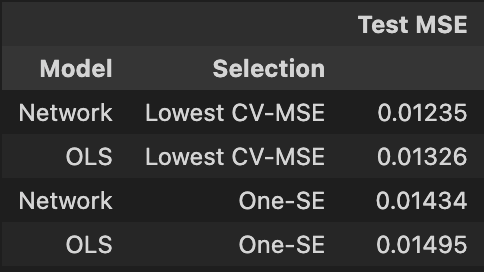
\includegraphics[width=\linewidth]{Results/Regressor/TS1.png}
    \caption{Test MSE for the lowest mse model and the chosen one se model}
    \label{fig:TS1}
\end{figure}
\FloatBarrier
\subsubsection{Second CV Gridsearch}
\begin{figure}[htbp]
    \centering
    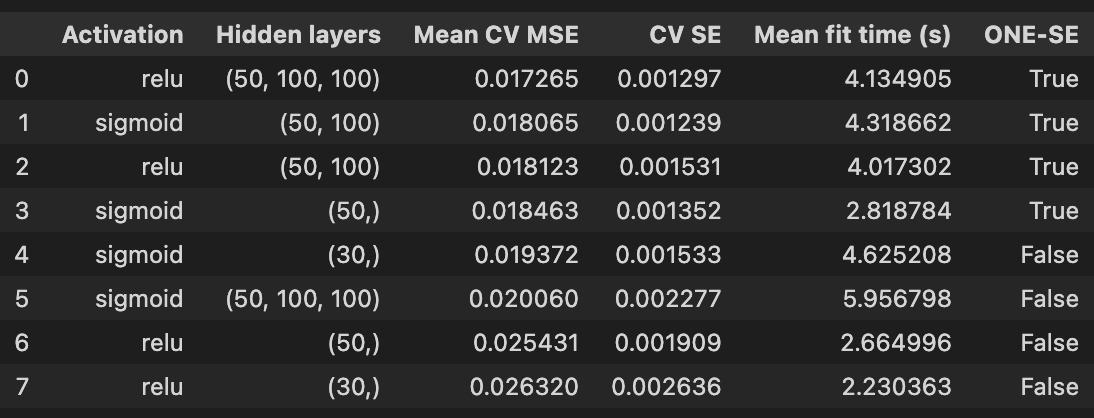
\includegraphics[width=\linewidth]{Results/Regressor/MS21.png}
    \caption{$\mathbf{Second CVGridSearch}:$ All model scores with standard error and mean fit time, along with a One SE validation for each model, with the lowest CV MSE as reference}
    \label{fig:MS21}
\end{figure}
\begin{table}
    \centering
    \caption{Vanishing Gradients}
    \label{tab:VanishGrad}
    \begin{tabular}{lc}
        \hline
        Layer & L2 Norm$(dW, db)$ \\
        \hline
        1 & $0.00976$ \\
        2 & $0.01524$ \\
        3 & $0.01065$ \\
        4 & $0.03032$ \\
    \end{tabular}
\end{table}

\FloatBarrier
\subsubsection{Third CV Gridsearch}
\begin{figure}[htbp]
    \centering
    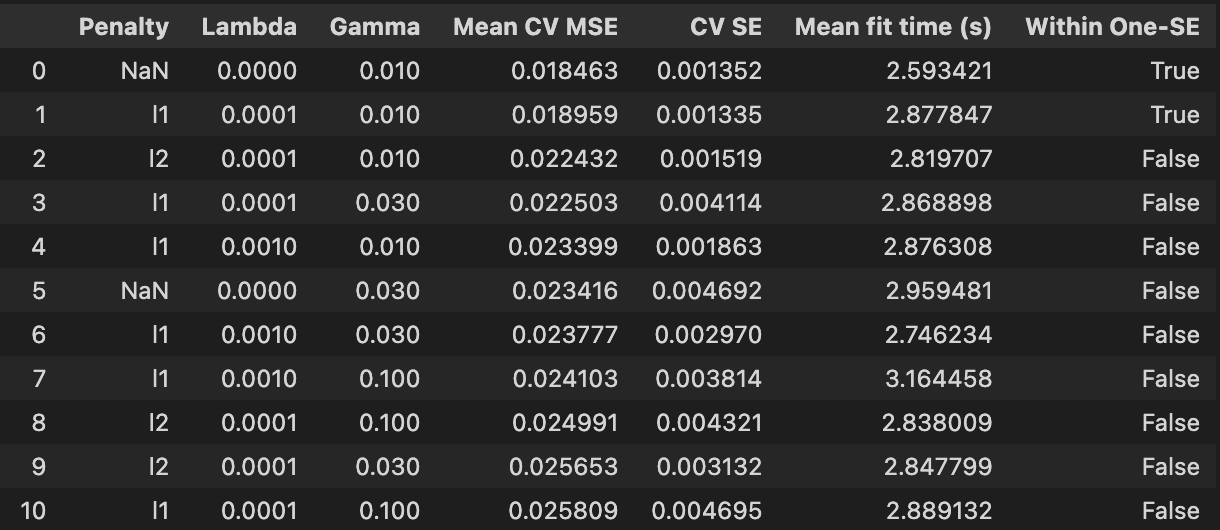
\includegraphics[width=\linewidth]{Results/Regressor/MS31.png}
    \caption{$\mathbf{Third CVGridSearch}:$ The 10 first model scores with standard error and mean fit time, along with a One SE validation for each model, with the lowest CV MSE as reference}
    \label{fig:MS31}
\end{figure}

\begin{figure}[htbp]
    \centering
    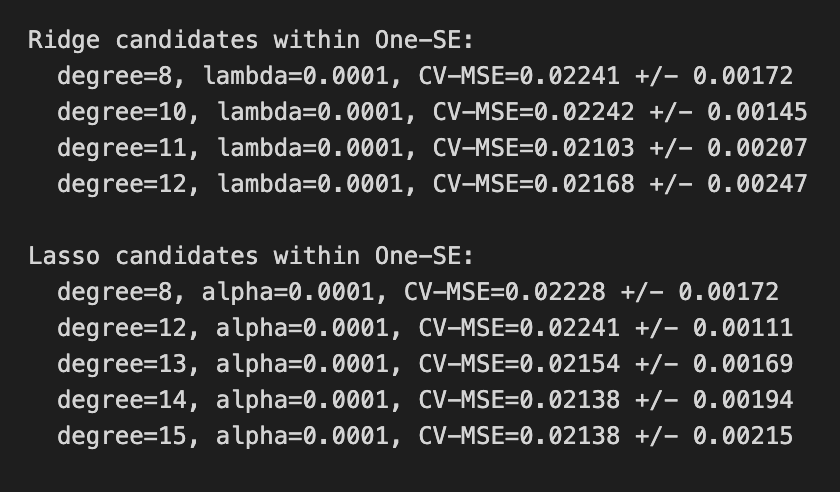
\includegraphics[width=\linewidth]{Results/Regressor/LR1.png}
    \caption{$\mathbf{Ridge and Lasso}:$ All models within one One SE, with the lowest CV MSE as reference}
    \label{fig:LR1}
\end{figure}


\begin{figure}[htbp]
    \centering
    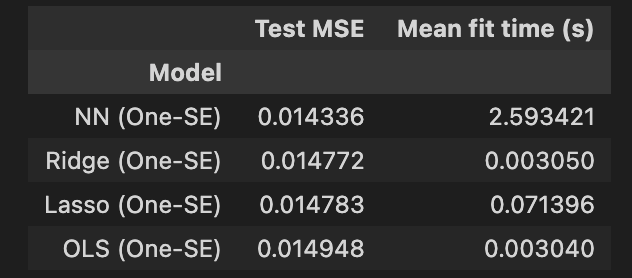
\includegraphics[width=\linewidth]{Results/Regressor/TS2.png}
    \caption{$\mathbf{Test set}:$ All chosen One SE models evaluated on the test set, once}
    \label{fig:TS2}
\end{figure}
\FloatBarrier
\subsection{NeuralNetClassifier}
\subsubsection{StratifiedKfold}
\subsubsection{Logistic Regression}
\subsubsection{GridsearchCV}
\begin{figure}[htbp]
    \centering
    \includegraphics[width=\linewidth]{\detokenize{Results/Class/HMC_B.png}}
    \caption{$\mathbf{Heatmap}:$ Containing the best model from cross validation, in red roddet lines, and two One-SE models}
    \label{fig:HMCB}
\end{figure}
\begin{figure}[htbp]
    \centering
    \includegraphics[width=\linewidth]{\detokenize{Results/Class/HMC_2.png}}
    \caption{$\mathbf{Heatmap}:$ Containing one One-SE model}
    \label{fig:HMC1}
\end{figure}
\begin{figure}[htbp]
    \centering
    \includegraphics[width=\linewidth]{\detokenize{Results/Class/HMC_3.png}}
    \caption{$\mathbf{Heatmap}:$ Containing two One-SE models}
    \label{fig:HMC2}
\end{figure}

\FloatBarrier
\subsubsection{Test Set once}
\begin{figure}[htbp]
    \centering
    \includegraphics[width=\linewidth]{\detokenize{Results/Class/CM1.png}}
    \caption{$\mathbf{Confusion Matrix}:$ cross val predict}
    \label{fig:CM1}
\end{figure}
\begin{figure}[htbp]
    \centering
    \includegraphics[width=\linewidth]{\detokenize{Results/Class/CM2.png}}
    \caption{$\mathbf{Confusion Matrix}:$ Best model applied on test data}
    \label{fig:CM2}
\end{figure}
